% Gere o PDF com o comando pdflatex, e o SVG com o comando
%
%  $ inkscape -l fig.svg source.tex
\documentclass{standalone}
\usepackage{tikz}

\begin{document}

    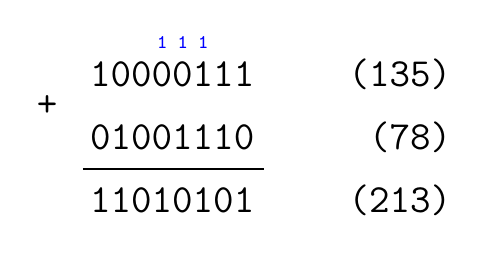
\begin{tikzpicture}
        \node[anchor=east] at (5.55, 3.4) { \scriptsize \textcolor{blue}{\texttt{1  1  1  }} };
        \node[anchor=east] at (6, 3) { \Large \texttt{10000111} };
        \node[anchor=east] at (8.5, 3) { \Large \texttt{(135)} };
        \node[anchor=east] at (6, 2.2) { \Large \texttt{01001110} };
        \node[anchor=east] at (8.5, 2.2) { \Large \texttt{(78)} };
        \node[anchor=east] at (3.5, 2.6) { \Large \texttt{+} };

        \draw[thick] (3.7, 1.8) -- (6, 1.8);

        \node[anchor=east] at (6, 1.4) { \Large \texttt{11010101} };
        \node[anchor=east] at (8.5, 1.4) { \Large \texttt{(213)} };
    \end{tikzpicture}

\end{document}
